\documentclass[conf]{new-aiaa}
%\documentclass[journal]{new-aiaa} for journal papers
\usepackage[utf8]{inputenc}

\usepackage{graphicx}
\usepackage{amsmath}
\usepackage[version=4]{mhchem}
\usepackage{siunitx}
\usepackage{longtable,tabularx}
\setlength\LTleft{0pt} 

\title{Fly-Back of a Scramjet-Powered Accelerator}

 \author{
 	Sholto O. Forbes-Spyratos%
 	\footnote{Ph.D. Candidate, Centre for Hypersonics, School of Mechanical and Mining Engineering. Member AIAA.}
 	\ ,  Michael P. Kearney
 	\footnote{Lecturer, School of Mechanical and Mining Engineering.}
 	\ ,  Michael K. Smart
 	\footnote{Professor, Centre for Hypersonics, School of Mechanical and Mining Engineering. Senior Member AIAA.}
 	\ and   Ingo H. Jahn
 	\footnote{Lecturer, Centre for Hypersonics, School of Mechanical and Mining Engineering. Member AIAA.}
 	\\
 	{\normalsize\itshape
 		The University of Queensland, Queensland, Australia, 4072}\\
 }

\begin{document}

\maketitle

\begin{abstract}

\end{abstract}

\section{Nomenclature}

{\renewcommand\arraystretch{1.0}
\noindent\begin{longtable*}{@{}l @{\quad=\quad} l@{}}
$A$  & amplitude of oscillation \\
$a$ &    cylinder diameter \\

\end{longtable*}}

\section{Introduction}

The decreasing size and cost of satellites is driving an upsurge in the number of small satellite launches\cite{Faa&Ast&Comstac2015}. Many of these small satellites require custom orbits which are specified by the satellite manufacturer, and have small launch windows. Satellites which form part of constellations are particularly sensitive to launch windows due to the requirement for them to fit into a specific orbital schedule\cite{Crisp2015}. Launchers which can deliver a small payload into a custom orbit, at short notice, are in increasing demand, and are being developed by a number of organisations. These small satellite launchers offer the user flexibility in orbit and launch schedule, at comparable cost-per-kg to piggybacking on larger launches. Currently all (CHECK) small launchers are expendable, however there is a push toward developing reusable small satellite launchers to reduce costs and improve turnaround times.

The development of reusable launch systems has recently flourished, led by SpaceX, and fuelled by the need to decrease launch costs and turnaround times. Incorporating reusability into the design of small satellite launchers is complicated, due to the scaling difficulties posed by the additional systems needed for reusability. 
The University of Queensland and Hypersonix (Check full name, eg LTD etc) are developing a rocket-scramjet-rocket multi stage launch system for small satellite launches, incorporating the SPARTAN scramjet-powered accelerator. 
The use of a scramjet engine improves the efficiency of the SPARTAN compared to rocket-powered vehicles, and eliminates the necessity for oxidiser to be carried on board. Carrying only fuel on board the vehicle allows the SPARTAN to have a design similar to a traditional aircraft, including avionics and landing gear. The aerodynamic capabilities and avionic systems of the scramjet stage allow it to return to its initial launch site, and land horizontally on a traditional runway. After landing, the vehicle will be checked and re-fuelled, and will then be ready to launch again. The increased reusability that this will afford over similarly sized launch systems will enable the cost-per-kg of launch to be reduced. 

\begin{figure}
\centering
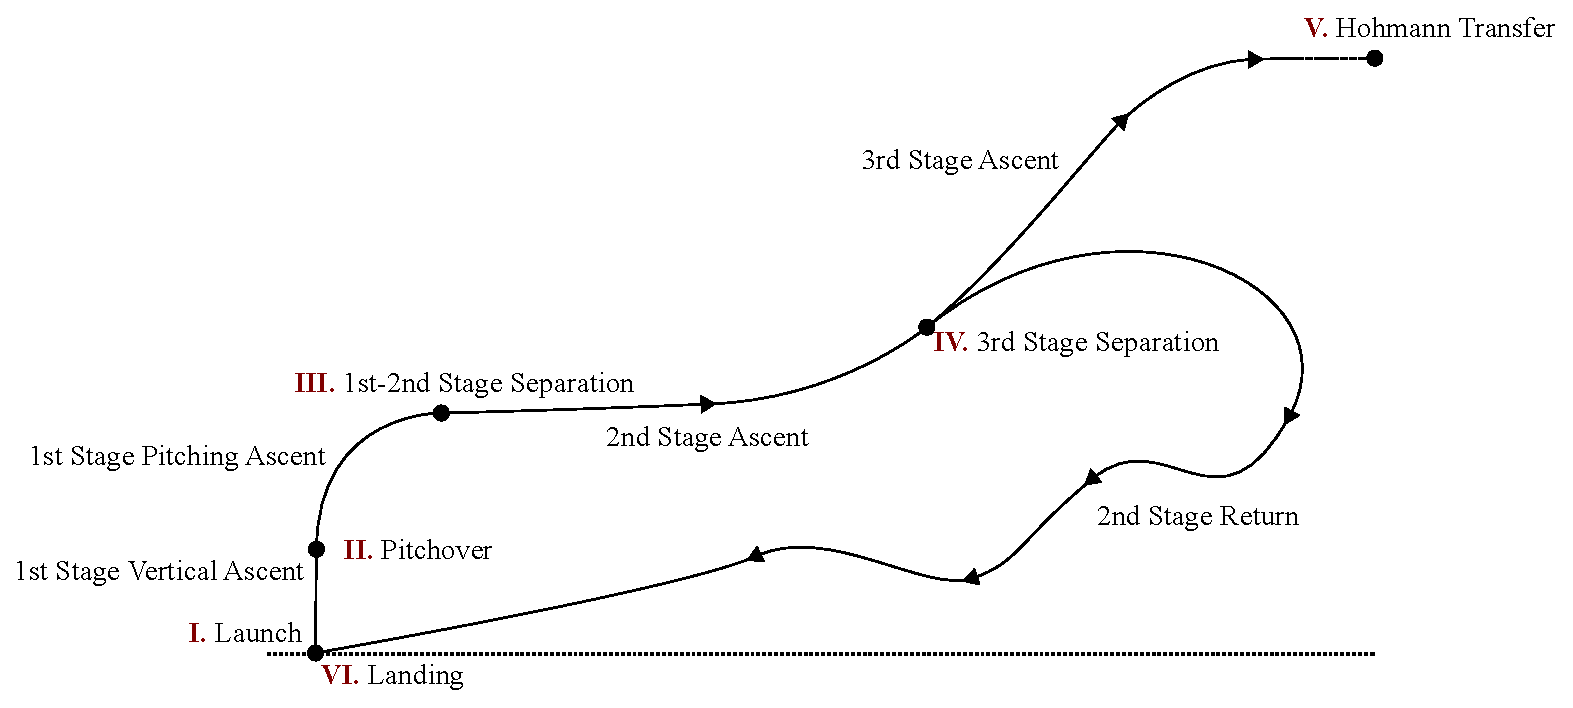
\includegraphics[width=0.9\linewidth]{Figures/Traj}
\caption{}
\label{fig:Traj}
\end{figure}


The trajectory of the rocket-scramjet-rocket launch system is shown in Figure \ref{fig:Traj}. The system launches vertically under rocket power, and pitches over until close to horizontal flight. The SPARTAN separates from the first stage rocket at Mach 5, the minimum operable Mach number of the scramjet engines. The SPARTAN then accelerates until approximately Mach 9, at which time a pull-up manoeuvre is performed and the third stage rocket is released. The third stage rocket then accelerates out of the atmosphere and then performs a Hohmann transfer to the desired orbit. Meanwhile, the SPARTAN turns and flies back to the initial launch site. 
The launch ascent profile of the rocket-scramjet-rocket system incorporating the SPARTAN vehicle has been analysed and optimised in previous studies. However, the fly-back of the SPARTAN must be simulated to ensure that the full reusability of the SPARTAN is achievable. This fly-back is crucial to the feasibility of the system, and the amount of fuel necessary to perform the fly-back may have a large effect on the payload-to-orbit of the system. 

It is desirable for the SPARTAN to perform a minimum-fuel fly-back to the initial launch site, with the best-case scenario being for the fly-back to use no fuel at all. However, for a hypersonic trajectory a fully glide-back return flight is impractical due to the large initial velocity at the beginning of the fly-back trajectory. 
In previous studies, the maximum separation velocity for glide-back to be feasible has been found to be between Mach 3-4, with higher initial velocities requiring fly-back under power.

Powered fly-back may be achieved either through the use of the existing airbreathing engines, or by using additional engines added for the fly-back only. 
The addition of subsonic engines powering a constant velocity cruise-back phase allows the accelerator to return to base with a similar trajectory to that of a traditional aircraft, allowing the velocity and altitude of the accelerator to be precisely controlled. However, the addition of subsonic engines necessary for cruise-back increases the mass of the vehicle significantly, leading to decreased launch efficiency. 

The use of the existing hypersonic airbreathing engines during the fly-back allows range to be added to the return trajectory, without the inclusion of additional engines. However, the hypersonic airbreathing engines may only be used within their operating region, and vary in thrust and efficiency dependent on flight conditions. This added complexity requires the fly-back trajectory to be optimised to minimise the fuel necessary to return to the launch site, and to ensure that the return of the vehicle under its own power is viable. 


Vehicles using high-speed airbreathing propulsion in return flight have been investigated in a study by Tsuchiya and Mori.  Tsuchiya and Mori investigate two conceptual launch vehicles; a vehicle powered solely by airbreathing propulsion returning after separation of an orbital stage at Mach 5.1, and an airbreathing/rocket vehicle returning after a separation at Mach 6.8. 
These boosters fly to a downrange distance of 600-625km from the launch site, and separate from the orbital accelerator at a dynamic pressure of 15kPa. At the start of their respective return trajectories, both boosters turn with a bank angle of 130-145$^\circ$. Both the fully-airbreathing and partially-airbreathing vehicles ignite their airbreathing engines for 'several tens of seconds' at approximately Mach 3.5, in order to extend the flight range of the vehicles and return to the initial launch site.


The SPARTAN has been shown to separate from its third stage rocket at Mach 9.1, at X dynamic pressure, and the SPARTANs scramjet engines must operate at hypersonic speeds of Mach 5.1 or higher. These conditions are considerably different than those studied by Tsuchiya and Mori. It is desired to invesigate the ability of the SPARTAN to return to the launch site following separation at high Mach number. 

The aim of this paper is to find the minimum-fuel fly-back trajectory for the SPARTAN vehicle, and to investigate the effects of stage separation location on the SPARTAN fly-back. 



\section{The SPARTAN}



\begin{figure}
\centering
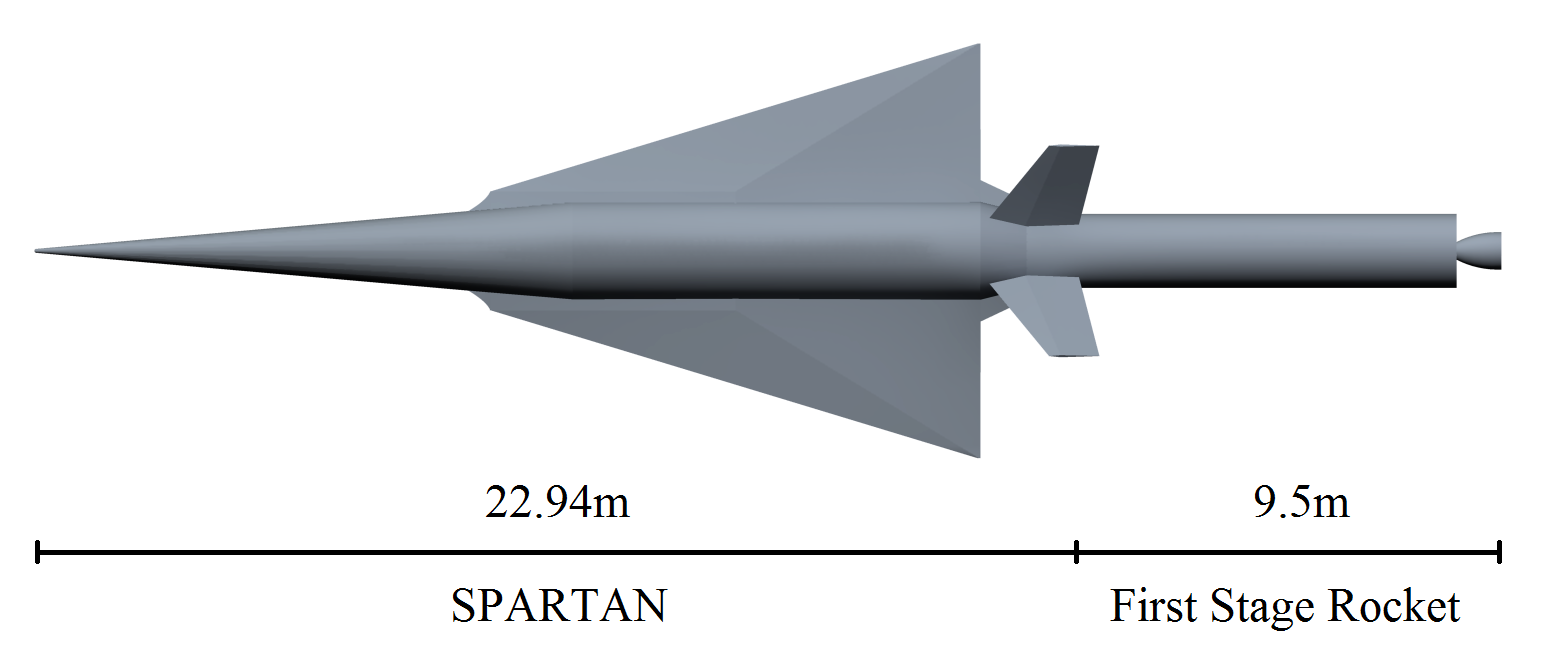
\includegraphics[width=0.7\linewidth]{Figures/NoInternal}
\caption{}
\label{fig:NoInternal}
\end{figure}
\begin{figure}
\centering
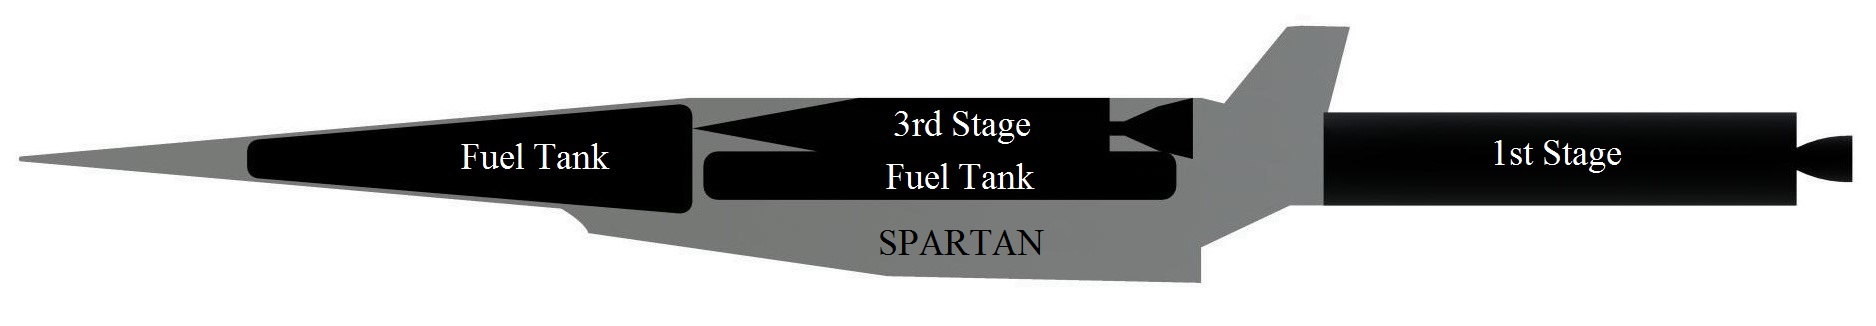
\includegraphics[width=0.7\linewidth]{Figures/INTERNALS}
\caption{}
\label{fig:INTERNALS}
\end{figure}


The SPARTAN is a scramjet-powered accelerator designed to operate between Mach 5 and Mach 9, as part of a rocket-scramjet-rocket multi-stage launch system. The SPARTAN is accelerated to Mach 5 by a rocket-powered first stage, at which point staging occurs. After the SPARTAN separates, the scramjet engines are used to accelerate. At the end of the SPARTANs acceleration the rocket-powered third stage is separated, which carries a payload to orbit. For the purposes of this study, the first stage is not investigated. Previously, the first stage has shown to deliver the SPARTAN to a range of separation points with only minor variation in performance. 

The SPARTAN has a total length of 22.94m, with a wingspan of XXX. The SPARTAN weights a total of 9819kg, including the third stage, and carries 1562kg of LH2 propellant. The SPARTAN is powered by four underslung C-REST scramjet engines, sized to a capture width of 0.65m.


%\subsection{Third Stage}

%The third stage rocket weighs a total of 3300kg, and is powered by a SpaceX LOX-kerosene Kestrel engine, weighing 52kg. The third stage rocket is protected while in-atmosphere by a heat shield weighing 130.9kg. The heat shield is constructed from a phenolic cork cylinder, carbon-carbon nose cone, and tungsten tip. When the third stage reached 10pa the heat shield is discarded, as aerodynamic heating is assumed to be negligible at this point. 
%\begin{figure}
	%\centering
	%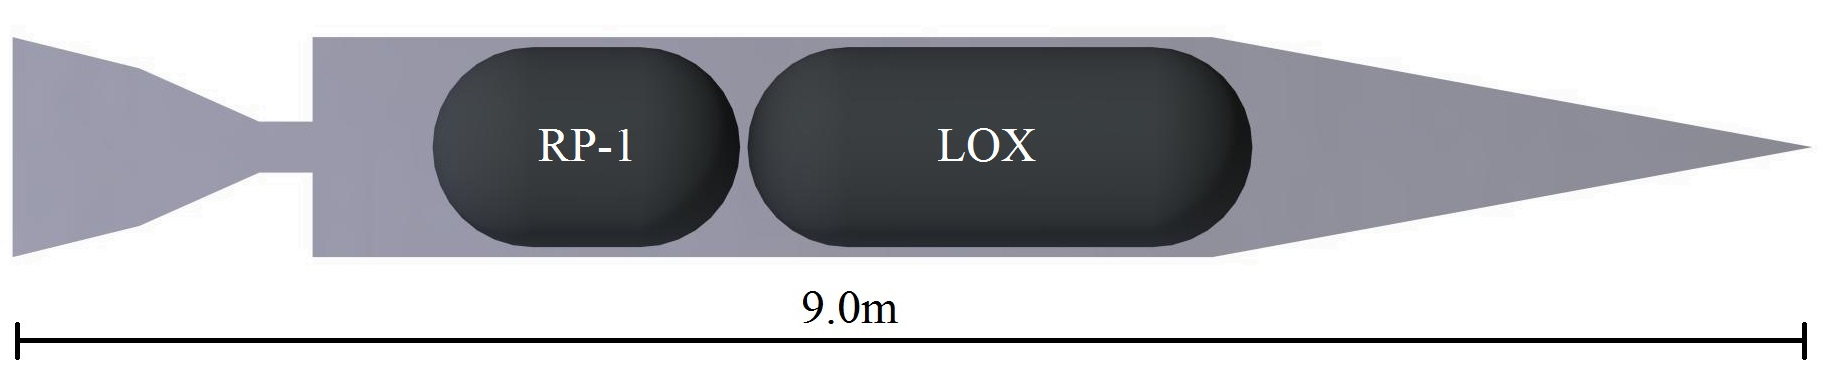
\includegraphics[width=0.7\linewidth]{Figures/3rdStage}
	%\caption{}
	%\label{fig:3rdStage}
%\end{figure}



\section{Aerodynamics}
 This study utilises CART3D to calculate the aerodynamics of the SPARTAN vehicle. CART3D is an inviscid CFD solver for the preliminary design of aerospace vehicles. CART3D utilises adjoint-based mesh refinement with a Cartesian cut-cells approach to produce a mesh refined iteratively to fit a flow solution. CART3D has been used to generate the aerodynamics of the SPARTAN vehicle due to its applicability over a wide Mach number range, and its robustness across multiple flow solutions. CART3D has previously been used to analyse hypersonic vehicles, and has shown good agreement with experimental data across multiple studies (CITATION HERE: sagerman,lee \& aftosmis).
 

SURFACE PLOTS OF CART3D CL AND CD VALUES

\section{Trajectory Optimisation}
The optimisation of the trajectories in this study were performed using LODESTAR. LODESTAR is a trajectory optimisation tool under development at The University of Queensland for hypersonic vehicle analysis. LODESTAR generates optimal trajectories given a target cost function, and sets of initial and end constraints. LODESTAR utilises the pseudospectral method optimisation software GPOPS-2. 


\subsection{Dynamic Model}

The SPARTAN is simulated in a geodetic rotational reference frame \cite{Josselyn2002a}: 

\begin{equation}
\dot{r} = v \, \sin \gamma
\end{equation}

\begin{equation}
\dot{\xi} = \frac{v \, \cos \gamma \, \cos \zeta}{r \, \cos \phi}
\end{equation}

\begin{equation}
\dot{\phi} = \frac{v\,\cos\gamma\,\sin\zeta}{r}
\end{equation}
\begin{equation}
\dot{\gamma} = \frac{T\,\sin\alpha}{m\,v}+ (\frac{v}{r}-\frac{\mu_E}{r^2 \,v})\,\cos\gamma + \frac{L}{m\,v}
+ \cos\phi[2\,\omega_E\, \cos\zeta + \frac{\omega_E^2\, r}{v}(\cos\phi\,\cos\gamma+\sin\phi\,\sin\gamma\,\sin\zeta)]
\end{equation}
\begin{equation}
\dot{v} = \frac{T\,\cos\alpha}{m}-\frac{\mu_E}{r^2}\,\sin\gamma - \frac{D}{m}
+ \omega_E^2 r\,\cos\phi(\cos\phi\,\sin\gamma-\sin\phi\,\cos\gamma\,\sin\zeta)
\end{equation}
\begin{equation}
\dot{\zeta} = -\frac{v}{r}\tan\phi\,\cos\gamma\,\cos\zeta +2\,\omega_E\,\cos\phi\,\tan\gamma\,\sin\zeta - \frac{\omega_E^2 r}{v\,\cos\gamma}\,\sin\phi \, \cos\phi\,\cos\zeta-2\omega_E\,\sin\phi 
\end{equation}

Where $r$ is the radius from the centre of Earth, $\xi$ is longitude, $\phi$ is latitude, $\gamma$ is flight path angle,$v$ is velocity and $\zeta$ is heading angle. The drag and lift of the SPARTAN are calculated using the standard aerodynamic coefficients;

\begin{equation}
F_d = \frac{1}{2} \, \rho \, C_D \, v^2 \, A ,
\end{equation}
\begin{equation}
F_L = \frac{1}{2} \, \rho \, C_L \, v^2 \, A .
\end{equation}

\section{Flyback Trajectory Analysis}
The flyback of the SPARTAN is optimised using LODESTAR. The flyback is optimised for minimum fuel flyback, with initial conditions constrained to be similar to the intended third stage release point, and end position constrained within XXXrad of the initial launch site, at XX,XX .  
The end of the trajectory is constrained to under XXXm altitude, and greater than XXXdeg trajectory angle. The end velocity is left unconstrained. It is assumed that for an optimal flyback trajectory, the end velocity will be minimised. 

\subsection{Reference Trajectory}

A reference fly-back trajectory is shown in Figures \ref{fig:Traj1}, \ref{fig:Traj2}, \ref{fig:Traj3} and \ref{fig:lon-lat}. This fly-back is initiated from 2.53 rad longitude, -0.135 rad latitude, 35km altitude, 3$^\circ$ trajectory angle, 2872m/s velocity and 102$^\circ$ heading angle. These conditions correspond to the approximate conditions of optimal third stage release. 

The SPARTAN starts at the maximum bank angle of 80$^\circ$, and sustains this bank angle for XXs. At this point, the altitude of the SPARTAN has decreased, and the vehicle is close to hitting the dynamic pressure of 50kPa. To avoid exceeding this limit, the bank angle is reduced to XX$^\circ$, allowing the vehicle to generate sufficient lift to begin increasing altitude. The bank angle in then increased again, to XX$^\circ$ at XXs. After this time, the bank angle is reduced gradually, reaching 10$^\circ$ at XXs, at which time the heading angle has reached XX$^\circ$. Soon after the bank angle has begun to reduce, at XXs flight time and Mach XX, the scramjet engines are throttled on. The SPARTAN burns for XXs, using a total of XXkg of fuel. The SPARTAN engines are throttled on close to the Mach number limit of 5.1, in order to maximise the specific impulse of the scramjet engines during burn. 


 At the end of the trajectory the SPARTAN pulls up, and lands at -1.2$^\circ$ trajectory angle, at 100m/s velocity. 

\begin{figure}
\centering
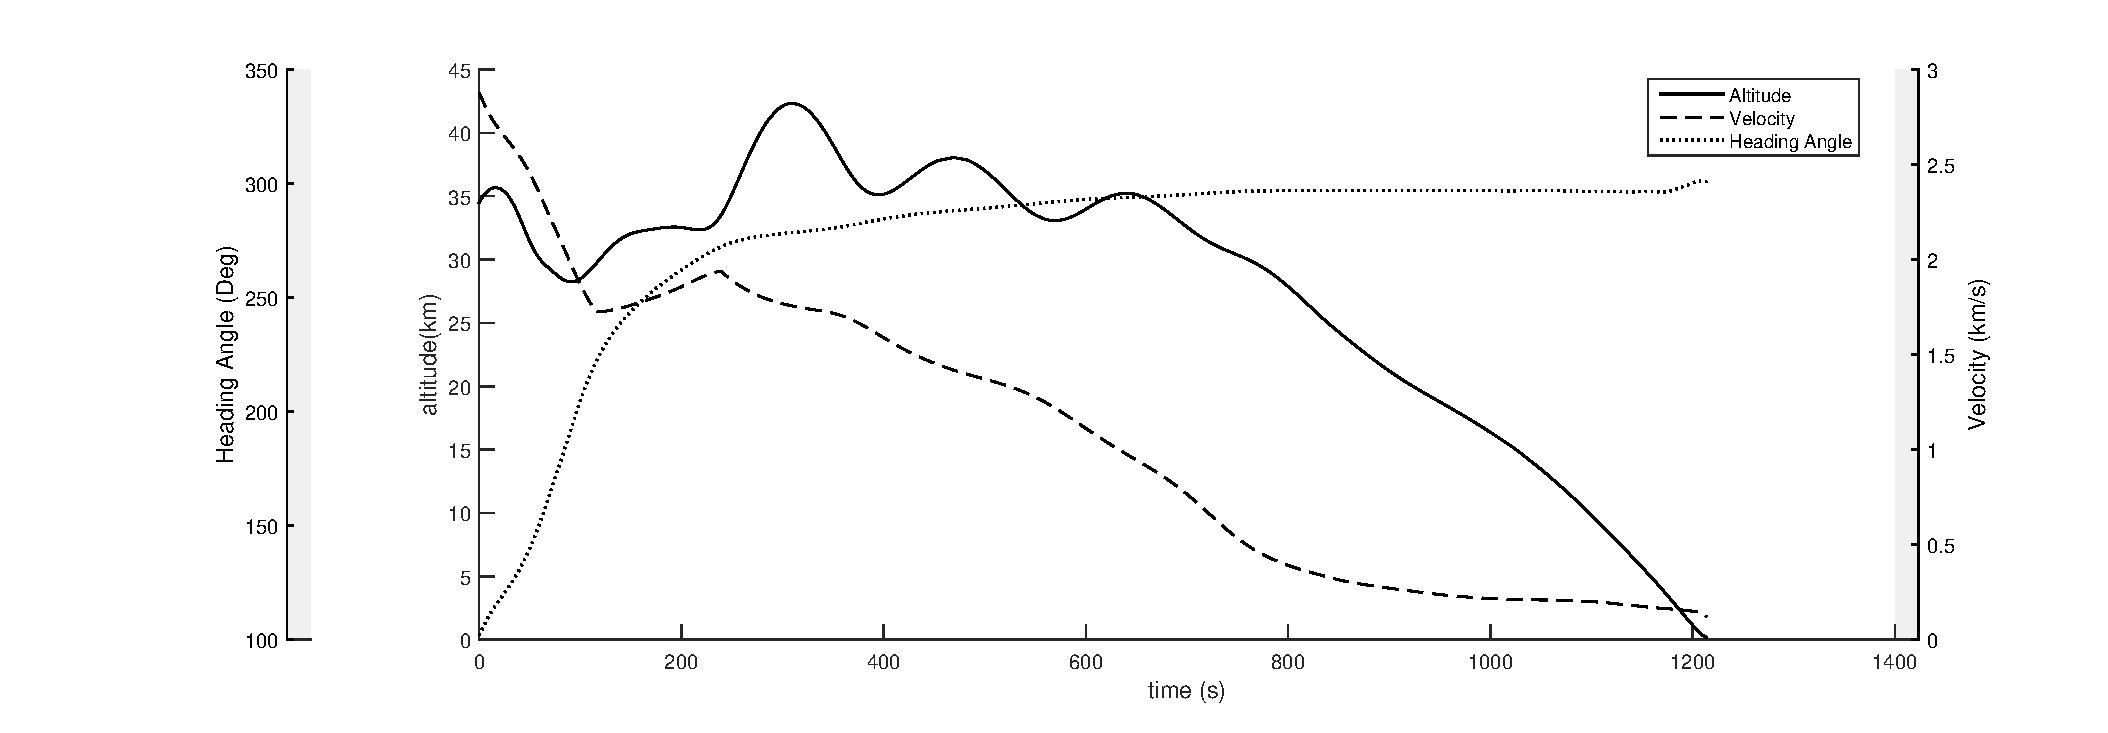
\includegraphics[width=0.9\linewidth]{Figures/Traj1}
\caption{Trajectory data for a SPARTAN return trajectory.}
\label{fig:Traj1}
\end{figure}
\begin{figure}
\centering
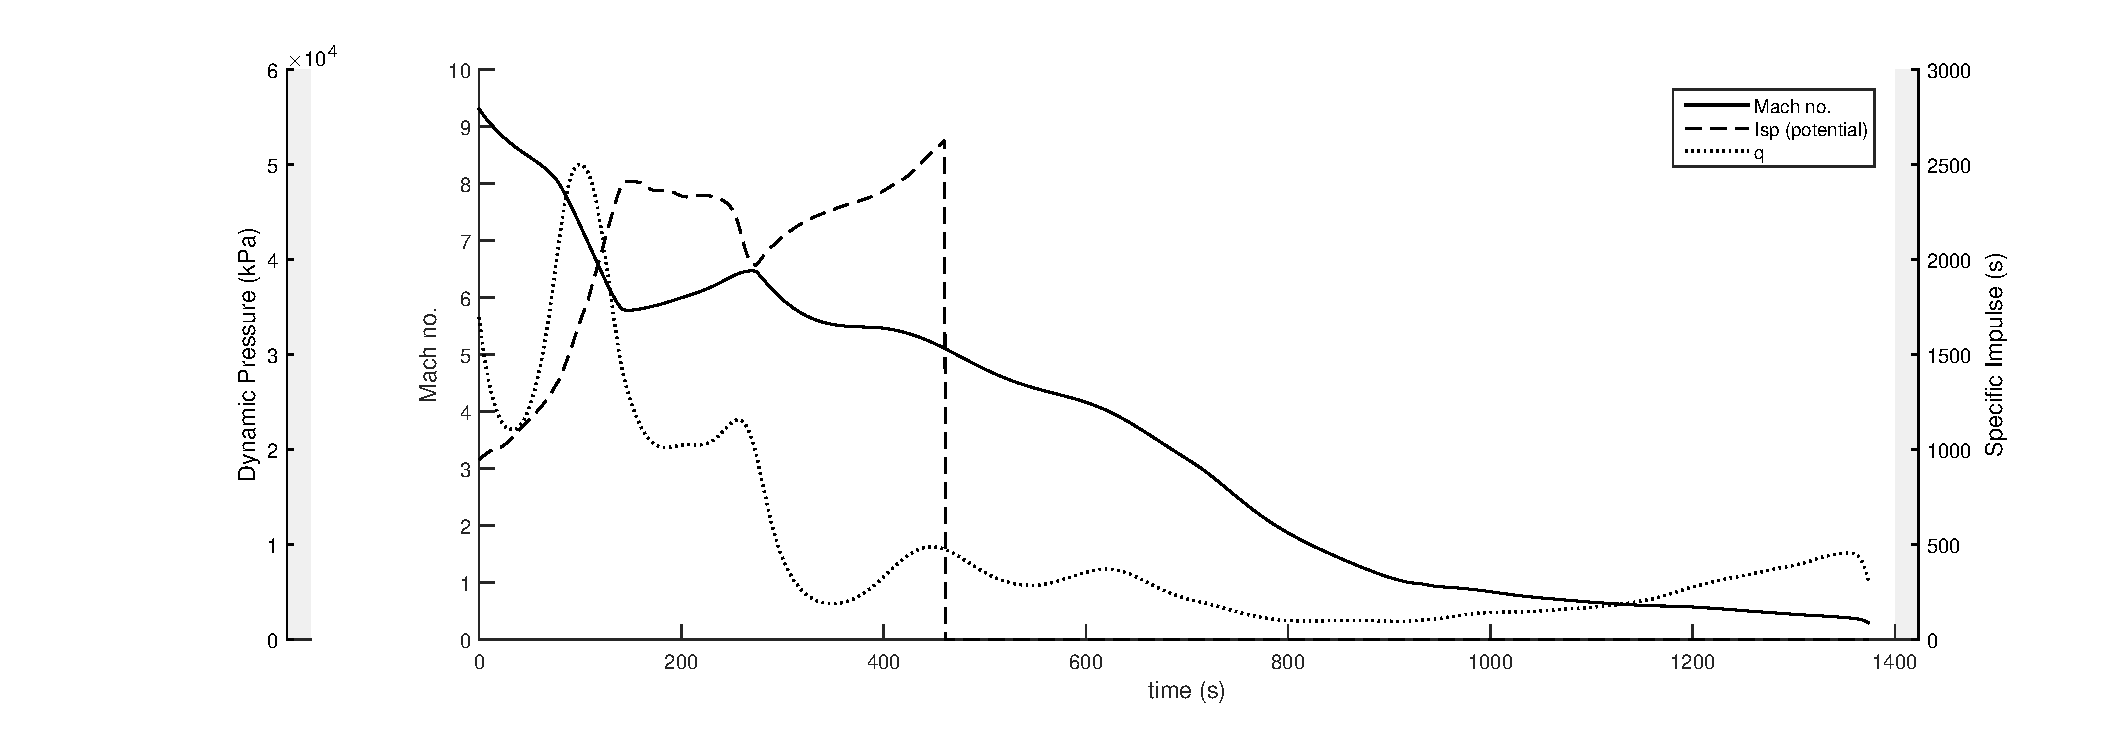
\includegraphics[width=0.9\linewidth]{Figures/Traj2}
\caption{Aerodynamic and performance data for a SPARTAN return trajectory.}
\label{fig:Traj2}
\end{figure}
\begin{figure}
\centering
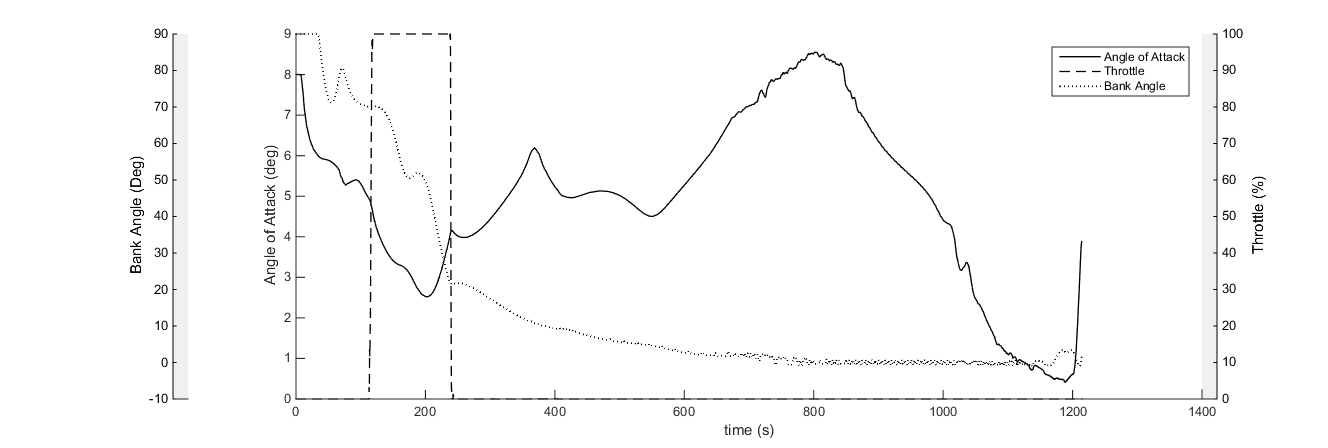
\includegraphics[width=0.9\linewidth]{Figures/Traj3}
\caption{Control data for a SPARTAN return trajectory.}
\label{fig:Traj3}
\end{figure}

\begin{figure}
\centering
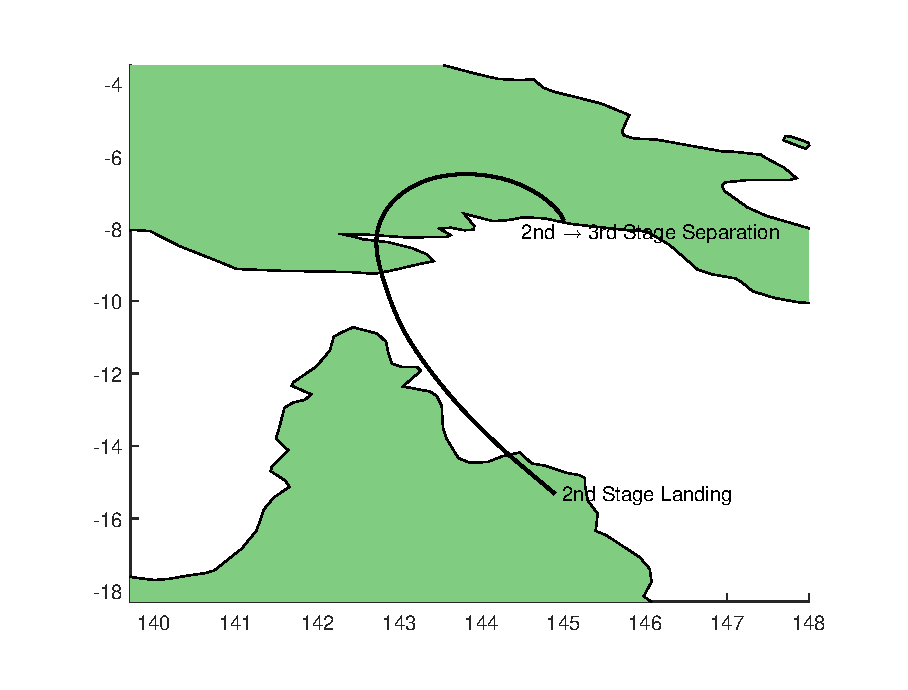
\includegraphics[width=0.7\linewidth]{Figures/lon-lat}
\caption{Ground track of a SPARTAN return trajectory.}
\label{fig:lon-lat}
\end{figure}


\subsection{Release Point Sensitivity}


\section{Conclusion}
The fly-back trajectory of the SPARTAN hypersonic vehicle has been investigated, from separation at XXX to landing at XXX. It has been found that the SPARTAN is capable of returning to its initial launch position, using XXkg of fuel. The SPARTAN lands at XXm/s.  

This study indicates that the launch of small satellites using a hypersonic vehicle which separates at Mach number greater than nine and then flies back to initial launch site is feasible. 

\section*{Acknowledgments}


\bibliography{library}

\end{document}
